% Chapter Template
\chapter{Data processing and structure} % Main chapter title

\label{Chapter3} % Change X to a consecutive number; for referencing this chapter elsewhere, use \ref{ChapterX}

%----------------------------------------------------------------------------------------
%	SECTION 1
%----------------------------------------------------------------------------------------

\section{Combining data sources}

This project used three main data sources, which need to be queried, filtered and combined to prepare the data for use in the models. When working with hundred of thousands of rows, the efficiency of the code is very important. Iterating through those rows might be necessary at times but will increase the time exponentially as compared to using vectorizing methods were possible. The three data sources were all in a different format. Measurement data from IMO was in text files, elevation data was in GeoTiff and reanalysis data from CARRA was in a GRIB format. To use the data to train, these three data sources needed to be combined into one file. This was done based on the measurement data from the IMO. A limit was set on the average wind speed and it was used to select measurement points. Along with the average wind speed having to be above a certain limit, to make sure that the same weather for the same location is not duplicated, only the top wind speed in any given 48 hour period is selected. That is, for a data point to be included it must have been the highest wind speed in the previous and following 24 hours, so as to not describe the same weather multiple times. The data from IMO was supplied for 10 minute increments, while CARRA data is in 3 hour intervals. This means that to use the CARRA data to predict the measured values from IMO, temporal interpolation would need to be done. Along with the temporal interpolation, note that the CARRA data is given in a rectangular grid where the distance between each point is around 2.5km while the the information from the IMO is given at specific locations. The elevation information was given by a 20 by 20 rectangular grid that covers Iceland. When combining these data sources a selection of interpolation method needs to occur. The interpolation was linear, both temporally and spatially. This might influence the results but was not considered in this study.

\begin{figure}[h]
    \caption{A flow chart showing how data sources were combined}
    \label{fig:data_preprocessing_flow_chart}
    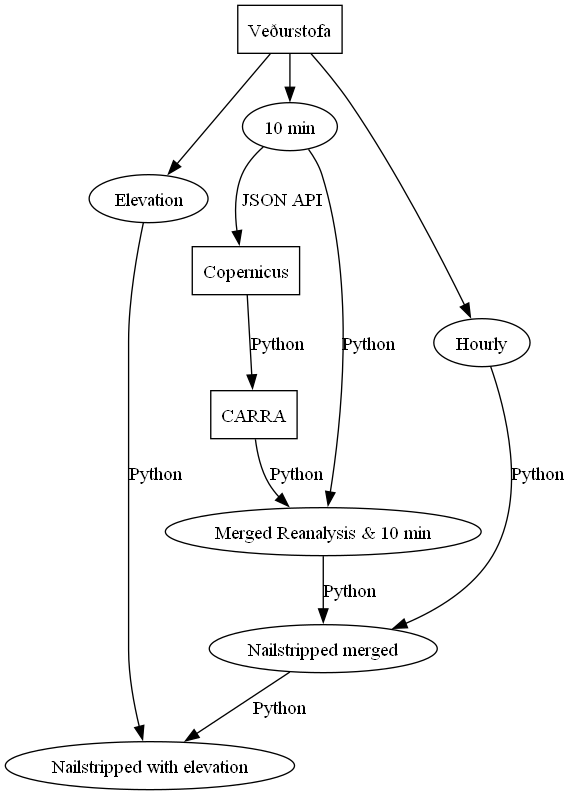
\includegraphics[scale = 0.5]{Figures/data-preprocessing-flow-chart-2024-04-08.png}
\end{figure}

The procedure of combining these sources was as follows and can be seen in Figure \ref{fig:data_preprocessing_flow_chart}. The measured data from the AWS is filtered by using a limit on the average wind speed. The gust factor generally drops with increased wind speed (although not always dependent on factors such as the landscape \cite{GNP_vidtal}). Even so being able to predict the gust factor is more important for higher average wind speed as there are the highest wind gusts. After this stripped dataset over every AWS has been created it is used to query the CARRA data by using their API. The CARRA API needs to be queried for given hours, days, months, years and a given area. That is, if queried for a given hour, it returns that hour for every day that is queried. Similarly if queried for a given day, it returns that day for every month. In light of these restraints, it was decided to query month by month. Querying only the days needed (both the days included in the 10 minute measurements and the days needed for interpolation if close to midnight) but every hour of the day (midnight, 03:00, 06:00, 09:00, midday, 15:00, 18:00 and 21:00) and then take these values and interpolate for the 10 minute values. After querying and downloading the data for the height levels and variables requested, points of interest are interpolated and values stored in a pandas dataframe. After this the downloaded data is discarded and the next month is queried. This drastically decreases the amount of data that needs to be stored as compared to downloading the entire area and keeping all the data points (goes from several terabytes to less than a gigabyte).

Once CARRA data has been merged with AWS data, using station and time columns, then this combined file needs to checked for nails. This is done by using the hourly data (which is supposedly error free). As the data has been filtered in for the highest average wind speed in a 48 hour interval, the hourly data can be used to find nails. The hourly data is combined with the merged AWS and 10 min data. Then filtering is applied on the average wind. If the average wind speed differs the rows are dropped. This can be used to look at which stations have high percentage error. This can be seen in Figure \ref{fig:error_count}.

\begin{figure}
    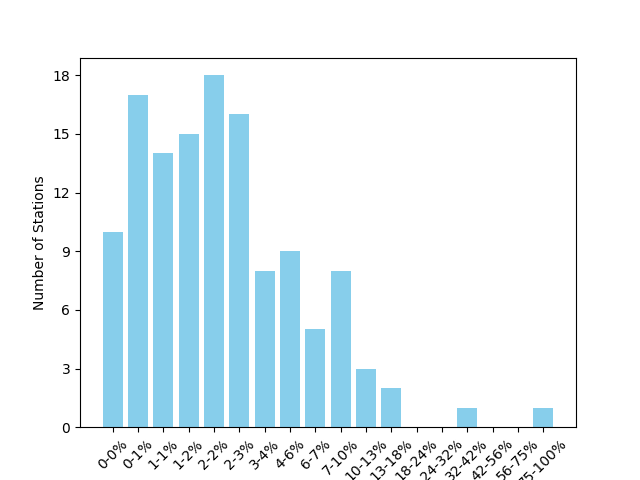
\includegraphics[scale=0.75]{Figures/error_count.png}
    \caption{The number of stations whose number of nails are in a certain percentage range of the overall}
    \label{fig:error_count}
\end{figure}

Figure \ref{fig:error_count} shows that most stations have nails in less that 10\% measurements. One has nails in 100\% of measurements. This is only because the number of measurements that matched previous criteria was 1.

The elevation data comes in a GeoTif file that covers Iceland. It is a rectangular grid of resolution 20 meters. For every point of interest (every weather station), the elevation of that given point along with other points surrounding the weather station is retrieved. For each point retrieved interpolation needs to be done. This is done in a similar manner to the interpolation of the CARRA data. Weights are assigned to each of the four points bounding the point of interest. These weights are then used to calculate the weighted average that represents the interpolated value. This information is included in the training data as the landscape is known to influence both the average wind and the gustiness \cite{GNP_vidtal}. 


\section{Data Structure}

Once data has been retrieved for all three sources and processed, including interpolating values, it needs to be made ready to use by the model, for both training, validation and test. Starting with a dataframe that contains measured information from AWS. This includes the average wind, the wind gust, wind direction along with the station number and coordinates. When selecting the CARRA data certain height levels are chosen. That is at which heights above ground the reanalysis parameters are requested. These present as separate lines in the CARRA dataframe. That is information for one observation is represented in as many lines as height levels requested in the reanalysis data. These rows need to be combined on the position (the weather station) and time so that each row contains all reanalysis information for a given measurement of a weather station. When this is done it is possible to combine the AWS IMO data and CARRA reanalysis data on the location and time columns. The last data source is the elevation. A couple of different sections of land around the weather stations have been looked at. A sector of a circle looking upwind, two sectors looking upwind and downwind and a circle around the point. In any case the points, that represent these sections, were selected like as shown in Code Listing \ref{code:sectorElevation}. That is a range of angles are defined based on the wind direction $d$ at some distance from the given point. This means that the resultant points (equal in number to the length of angleRange by k) form sectors at several distances from the given weather station.

\begin{lstlisting}[style = Python, caption = {Sector elevation points generated}, label = code:sectorElevation]
angles = [(angle + (90 - d)) * pi/180 for angle in angleRange]
length_rng = [(exp(i * log(n + 1)/ k) - 1) * 1000 
                for i in range(1, k + 1)]
points = np.array([[(X + l * cos(angle), Y + l * sin(angle))
                    for angle in angles] for l in length_rng])   
\end{lstlisting}

The result is a dataframe that has measured data from AWS, which gives us our target, reanalysis data from CARRA, which gives us weather variables to train on, and finally elevation points in the landscape to include in our training data. An example of what the data looks like can be seen in Table \ref{table:trainDataExample}.

\begin{table}[h]
    \caption{An example of data structure used with model}
    \label{table:trainDataExample}
    \resizebox{\textwidth}{!}{
    \centering
    \begin{tabular}{c|c|c|c|c|c|c|c}
         Ri\_01 & Ri\_12 & N\_01 & N\_12 & station\_elevation & relative\_corner & PC1 & ...\\\hline
         -1.18e+00 &  2.67e+04 & -8.57e-06 & 6.78e-05 & 3.34e+01 & 2.73e+00 & 1.36e+01 & ... 
    \end{tabular}
    }
\end{table}

Looking at Table \ref{table:trainDataExample} note that the last \nPCA columns represent the principle component analysis of the elevation data. Also note that the first four columns represent two variables that describe the stability of the air. These are the Richardson number ($Ri$)\cite{richardson_number_skybrary} and Brunt–Väisälä frequency\cite{brunt_vaisala_freq_eumtrain} ($N$). They are calculated using Equations (\ref{eqn:Ri}) and (\ref{eqn:N})\cite{mean_gust_HA_HO}. They are calculated using reanalysis data about the the weather at two different height levels. Thus $Ri_{01}$ refers to the Richardson number calculated between height levels 0 and 1. Exactly the same notation is used with the Brunt–Väisälä frequency. The height levels used were 15, 250 and 500 meters above the ground.

\begin{equation}
    \label{eqn:Ri}
    Ri = \frac{g \cdot dT \cdot dz}{T_{\textrm ave} \cdot dU^2} \unit{[]}
\end{equation}

\begin{equation}
    \label{eqn:N}
    N = \sqrt{\frac{g \cdot dT }{T_{\textrm ave} \cdot dz}} \unit{[Hz]}
\end{equation}

Here, $g$ is the acceleration due to gravity, $dT$ is the temperature difference between the two height levels, dz is the elevation difference, $T_{\textrm ave}$ is the average temperature (that is the average of the two temperatures in the height levels) and $dU$ is the wind speed difference between the two height levels. Both of these numbers provide some insight about the stability of the air. A lower value for the Richardson number indicates a higher turbulance. A typical range of values could be between 10 and 0.1, with values below 1 indicating significant turbulance\cite{richardson_number_skybrary}. When the square of the Brunt-Väisälä frequency is negative, then the air is unstable (an air parcel will move away from its original position)\cite{brunt_vaisala_freq_eumtrain}. These are derived factors from the reanalysis data and as such there shouldn't be a significant information gain using $Ri$ and $N$ as opposed to having the raw data. Including these factors instead of every reanalysis variable requested might speed up training as well as making the model more easily explainable with the use of Shapley values or other tools for explainability. Using Shapley a feature importance value is attributed to a given feature by creating all possible permutations of any possible length (up to number of features) and seeing how the predictions are skewed when the given parameter is included or excluded. This the needs to be done for all parameters. The time complexity of this is very high ($2^n$ coalitions)\cite{shapley_information}. Most implementations use some approximations, which still can take a considerable amount of time for models with a high parameter count and many examples.

